\documentclass[12pt]{article}
\usepackage[utf8]{inputenc}
\usepackage[a4paper, margin=1in]{geometry}
\usepackage{titlesec}
%\usepackage[style=ieee, backend=biber]{biblatex}
\usepackage{graphicx}
\usepackage{amsmath}
\usepackage{amssymb}
\usepackage{amstext}
\usepackage{enumitem}
\usepackage{siunitx}
\usepackage{array}
\usepackage{xcolor}
\usepackage{multirow}
\usepackage{hyperref}
\usepackage{tabularx}
\usepackage{booktabs}
\usepackage{soul}
\usepackage{fancyhdr}
\usepackage{setspace}
\usepackage{multicol}
\setlength{\columnsep}{.7cm}

\hypersetup{
    colorlinks=true,
    linkcolor=blue,
    filecolor=magenta,
    urlcolor=blue,
    pdftitle={aes670hw2},
    pdfpagemode=FullScreen,
    }
\urlstyle{same}

\newcolumntype{L}{>{$}l<{$}}  % Math mode table
\newcolumntype{R}{>{$}r<{$}}  % Math mode table
\newcolumntype{C}{>{$}c<{$}}  % Math mode table

\pagestyle{fancy}

\renewcommand{\sectionmark}[1]{%
\markboth{\thesection\quad #1}{}}
\fancyhead{}
\fancyhead[L]{\leftmark}
\fancyfoot{}
\fancyfoot[C]{\thepage}

\bibliographystyle{ieeetr}

\definecolor{Light}{gray}{.9}
\sethlcolor{Light}

\newcommand{\hltexttt}[1]{\texttt{\hl{#1}}}

\newcommand*{\problem}[2]{
    \begin{table}[ht]
    \centering
        \begin{tabular}{ | p{.1\linewidth} p{.9\linewidth} | }
            \hline
            \vspace{.3em}\textbf{\large#1:} & \vspace{.3em}\footnotesize{#2}\hspace{.2em}\vspace{.5em} \\ \hline
        \end{tabular}
    \end{table}
}

\newcommand\T{\rule{0pt}{2.6ex}}       % Top strut
\newcommand\B{\rule[-1.2ex]{0pt}{0pt}} % Bottom strut

\titleformat{\section}
  {\normalfont\fontsize{14}{15}\bfseries}{\thesection}{1em}{}

\titleformat{\subsection}
  {\normalfont\fontsize{12}{15}\bfseries}{\thesubsection}{1em}{}

\title{AES 770 Satellite Remote Sensing II

Smoke and Cloud Radiative Forcing}

\author{Mitchell Dodson}
\date{November 7, 2023}

\begin{document}

\maketitle

\vspace{-2em}

\begin{figure}[h!]
    \centering
    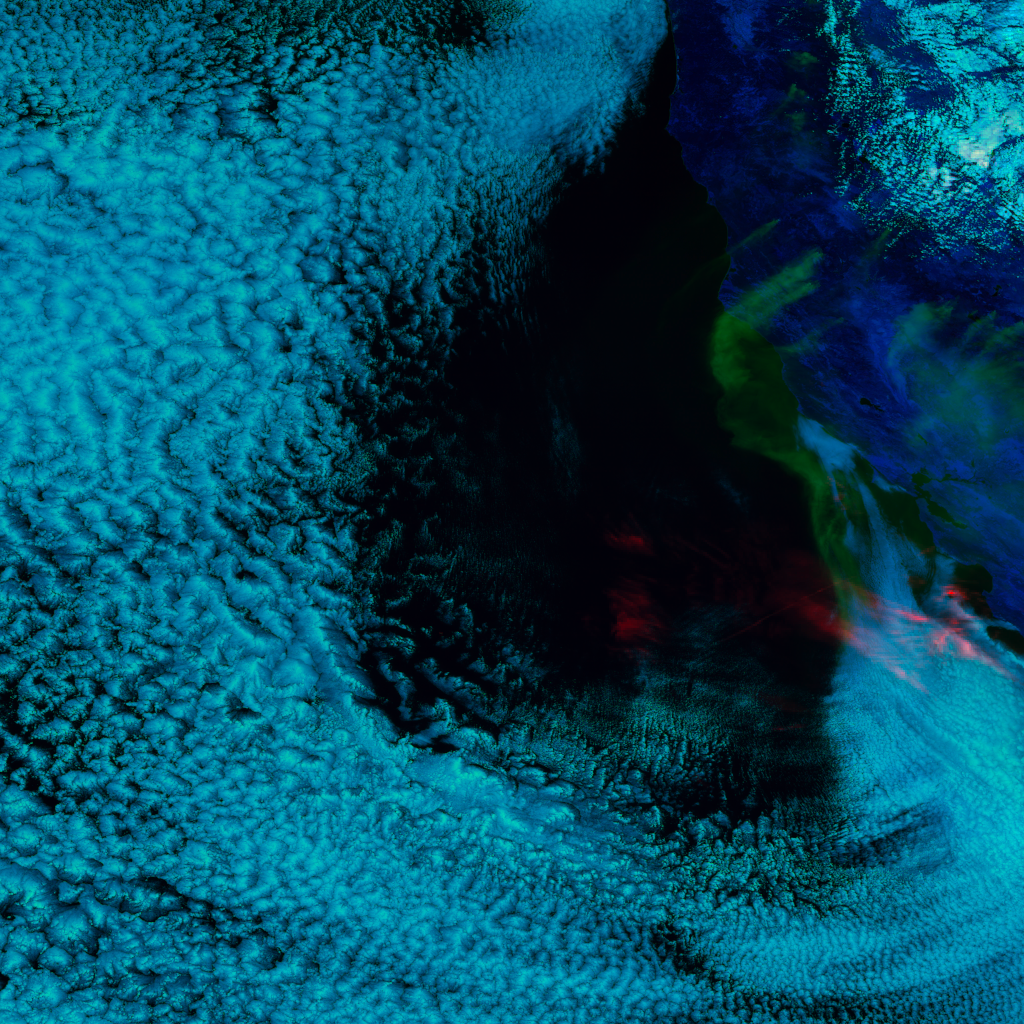
\includegraphics[width=.5\paperwidth]{figs/cover.png}
    \caption{GOES-17 ABI Truecolor RGB of the Region of Interest, captured on August 19, 2021 at 2137z. The scene shows widespread stratocumulus cover as well as thick wildfire smoke over the ocean, which is typical for the observations used in this report.}
    \label{cover}
\end{figure}

\vspace{-1em}

\section{Abstract}

In this report, I provide an assessment of the Cloud Radiative Forcing (CRF) and Aerosol Radiative Forcing (ARF) in both the longwave and shortwave spectral ranges using L2 Single-Scan Footprint (SSF) data from the Clouds and Earth Radiant Energy System (CERES) instrument, as well as co-located imager data from the Moderate Resolution Imaging Spectroradiometer (MODIS) instrument on the same satellite platforms, which are included with the SSF dataset. I focus on a Region of Interest (RoI) spanning $135^\circ W$ to $120^\circ W$ and $30^\circ N$ to $45^\circ N$, and the data I include consists of daytime overpasses from both the Terra and Aqua satellites between August 15 and August 25, 2021.


%\begin{multicols}{2}

\begin{figure}[h!]\label{fire-progression}
    \centering
    \begin{center}
        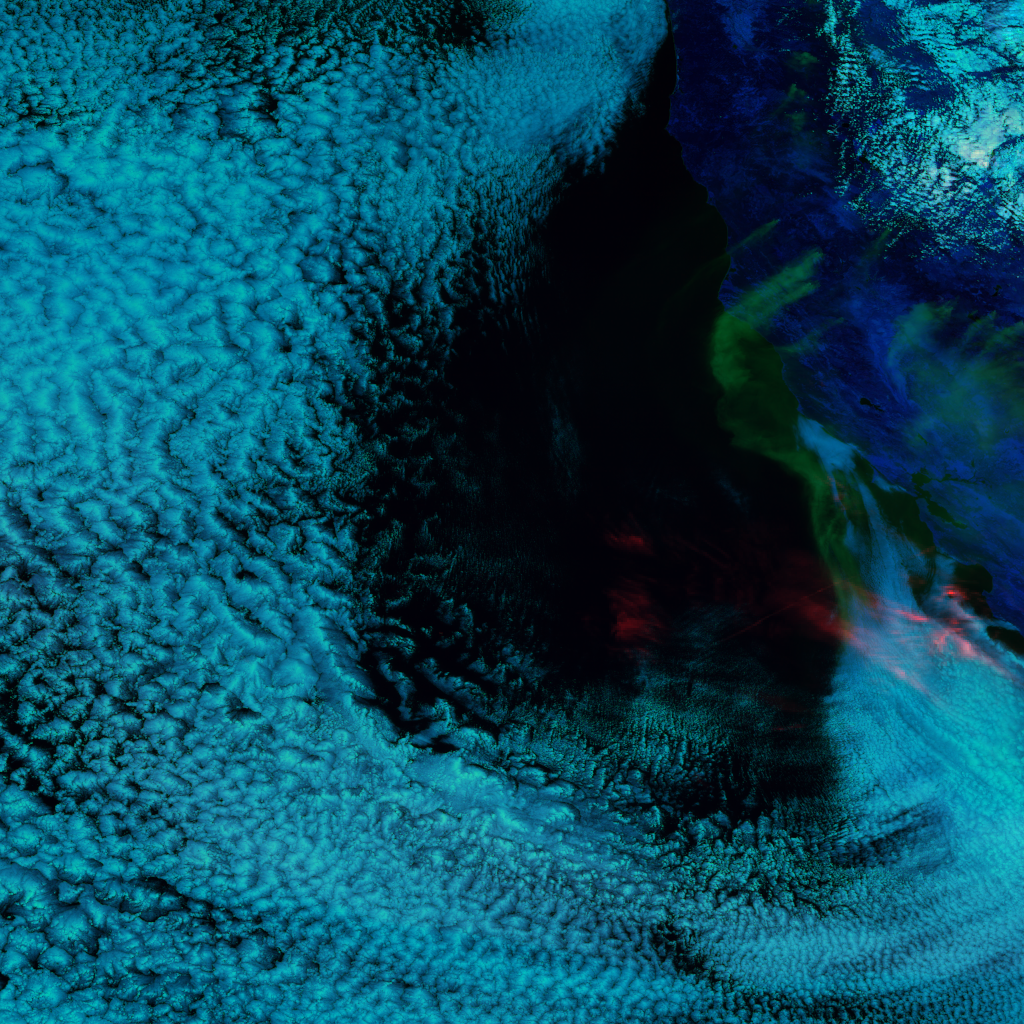
\includegraphics[width=.24\linewidth]{figs/abi_dcp_20210818-1912.png}
        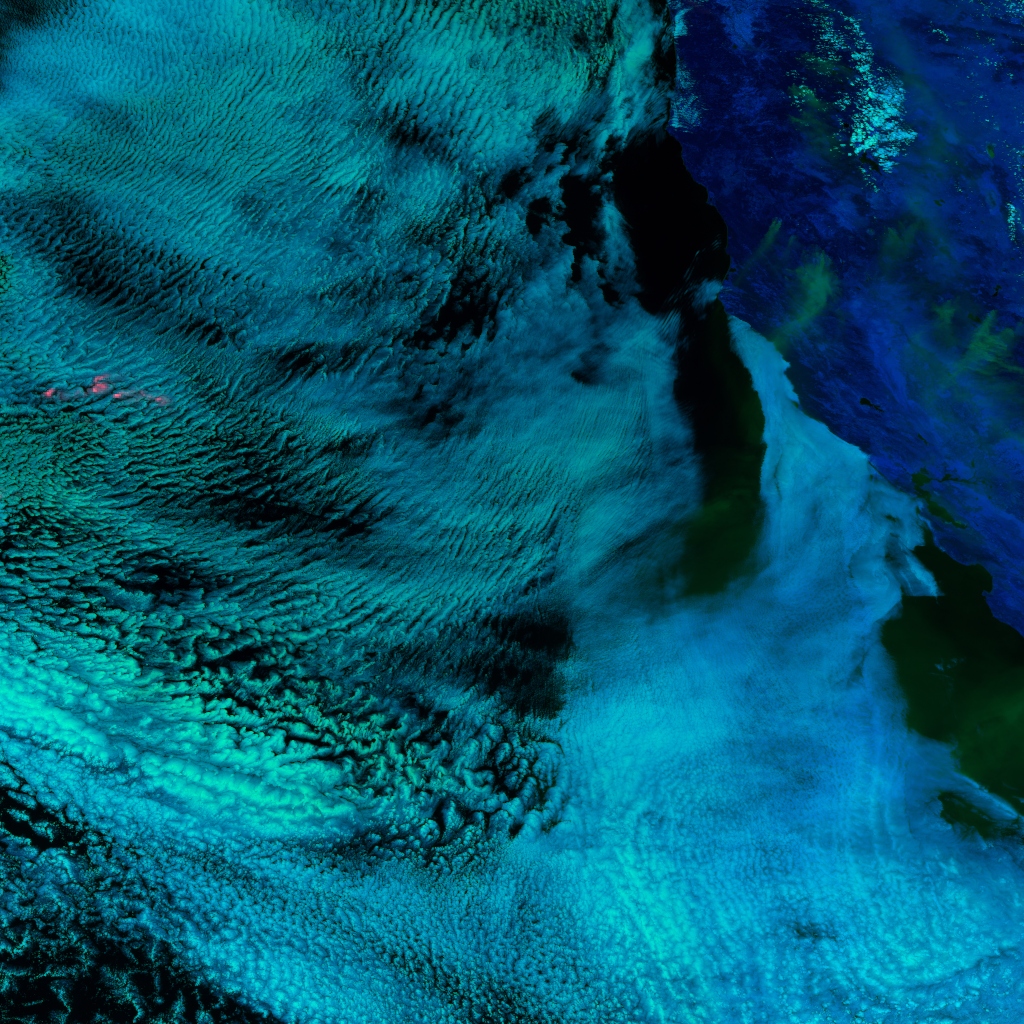
\includegraphics[width=.24\linewidth]{figs/abi_dcp_20210819-2137.png}
        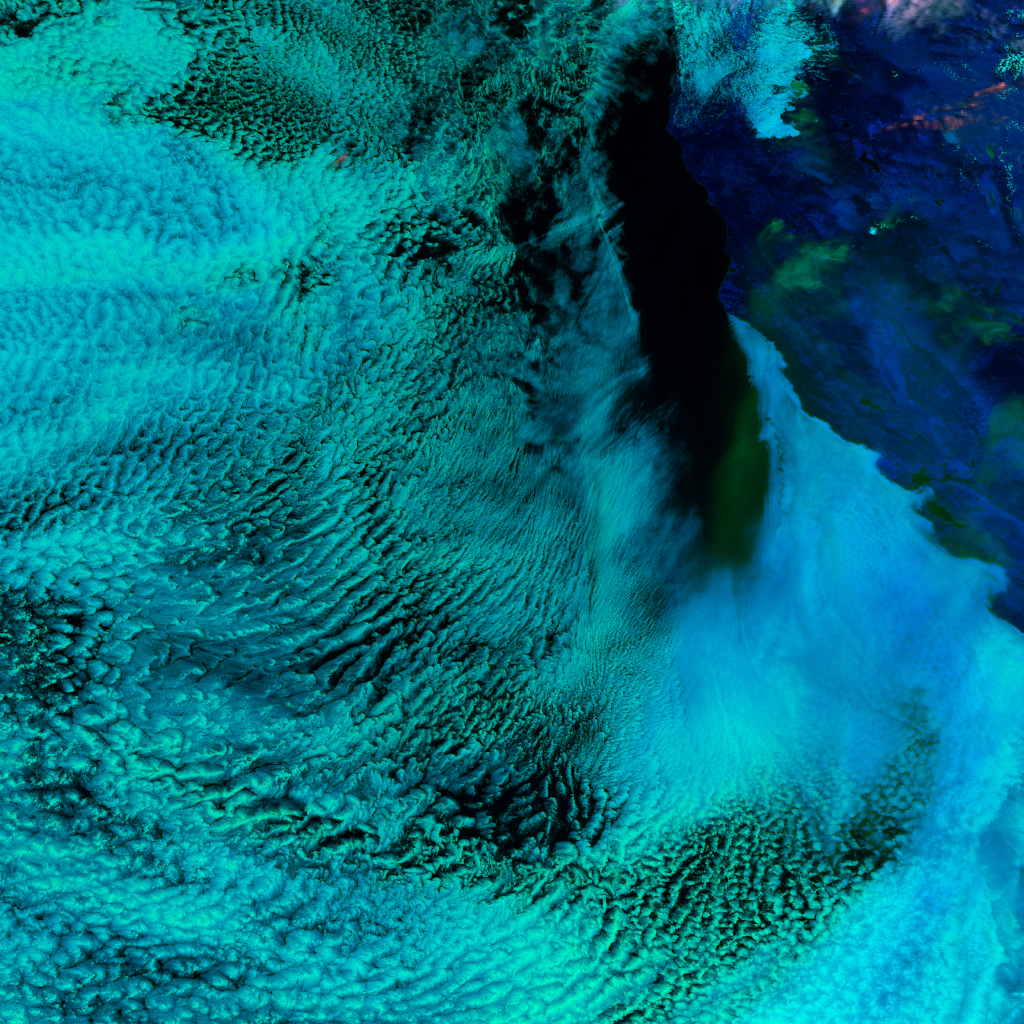
\includegraphics[width=.24\linewidth]{figs/abi_dcp_20210820-1900.png}
        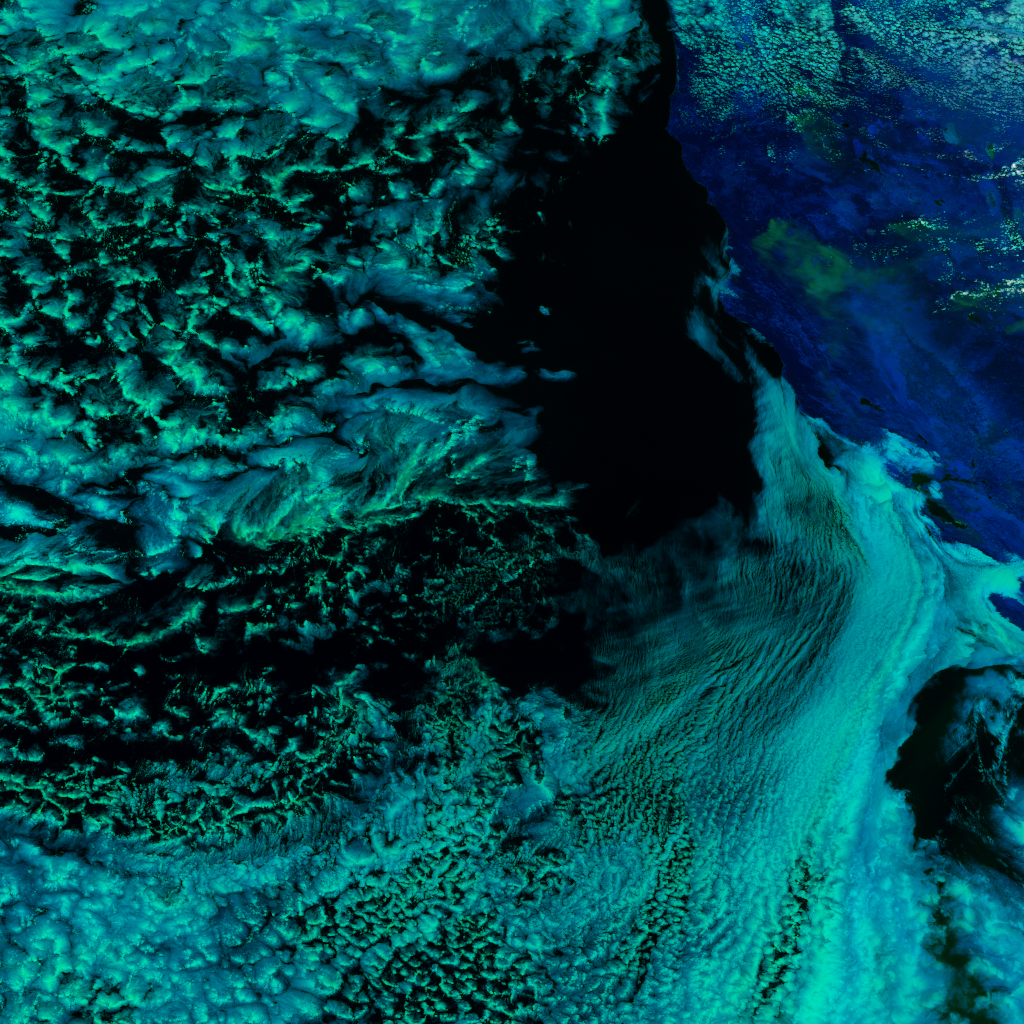
\includegraphics[width=.24\linewidth]{figs/abi_dcp_20210821-2125.png}

        \vspace{.2em}

        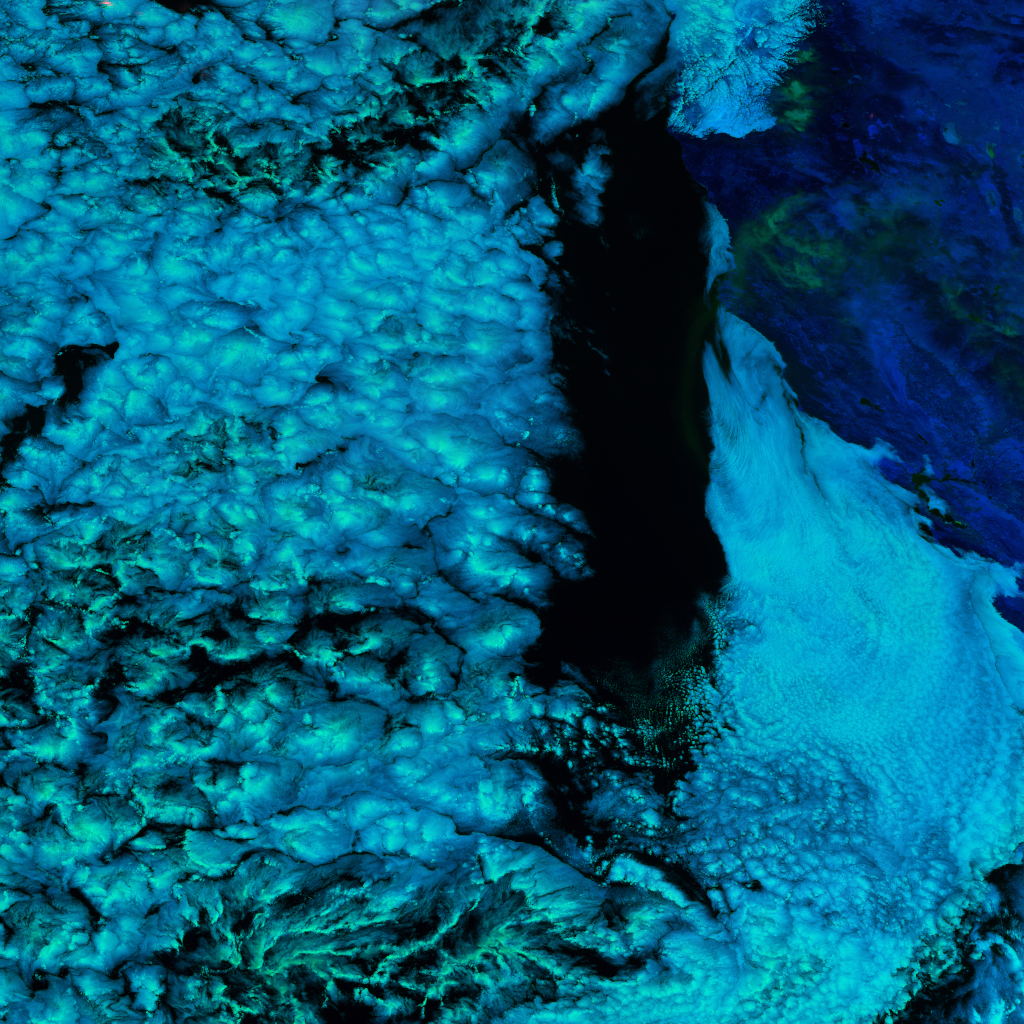
\includegraphics[width=.24\linewidth]{figs/abi_dcp_20210822-1848.png}
        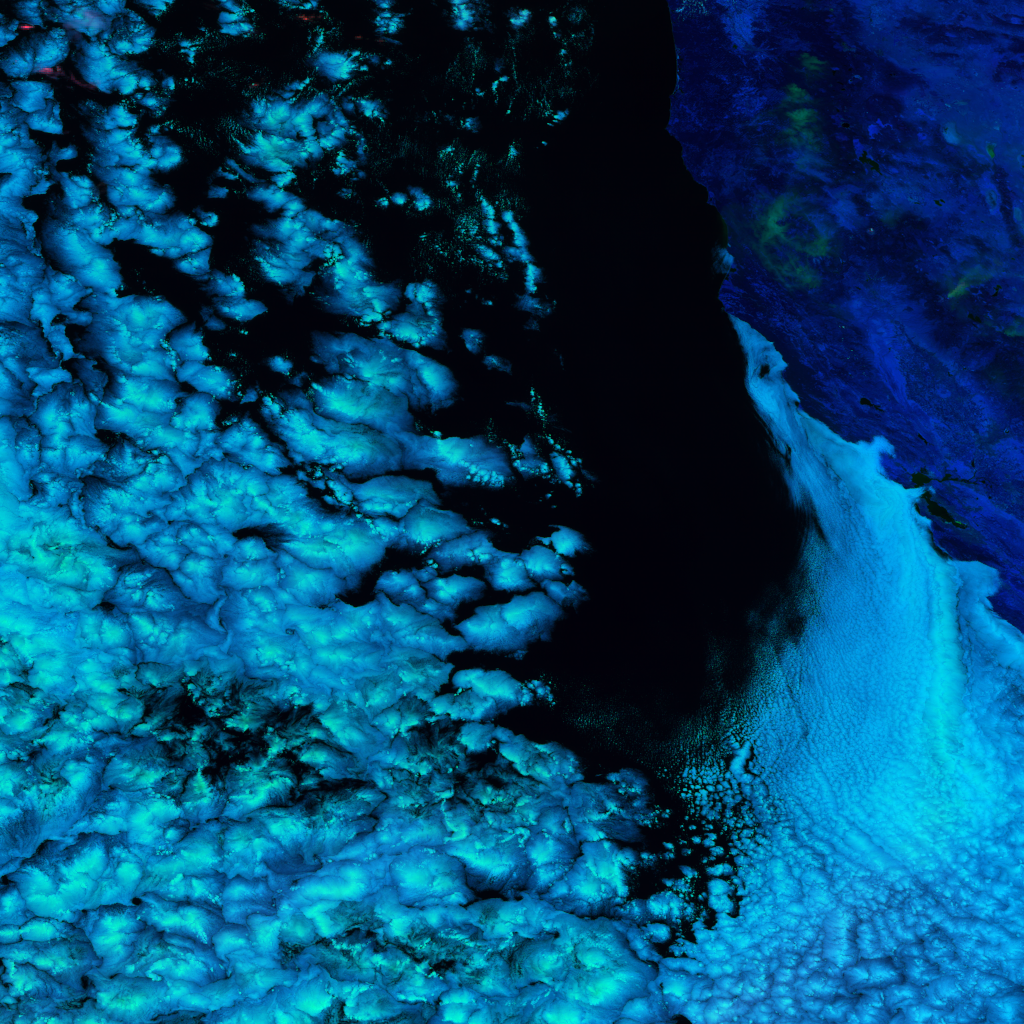
\includegraphics[width=.24\linewidth]{figs/abi_dcp_20210823-1931.png}
        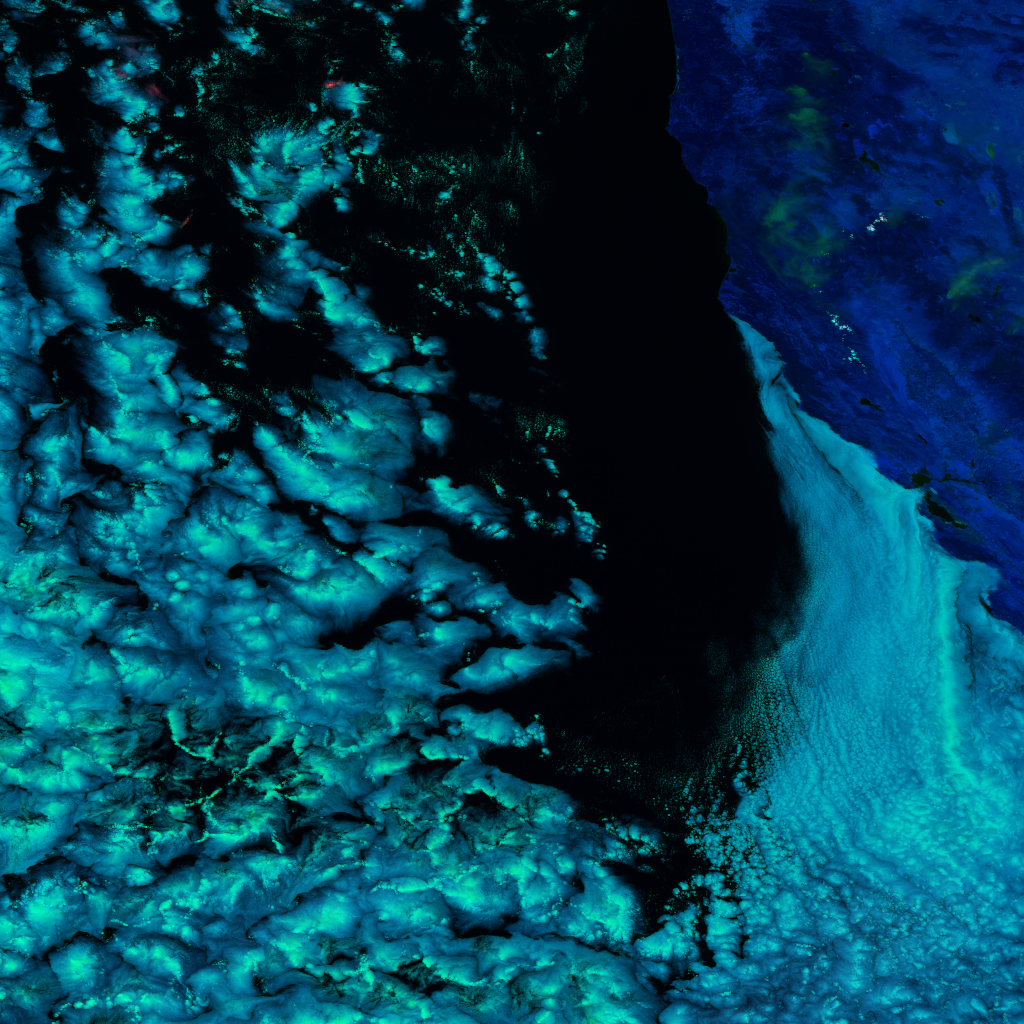
\includegraphics[width=.24\linewidth]{figs/abi_dcp_20210823-2113.png}
        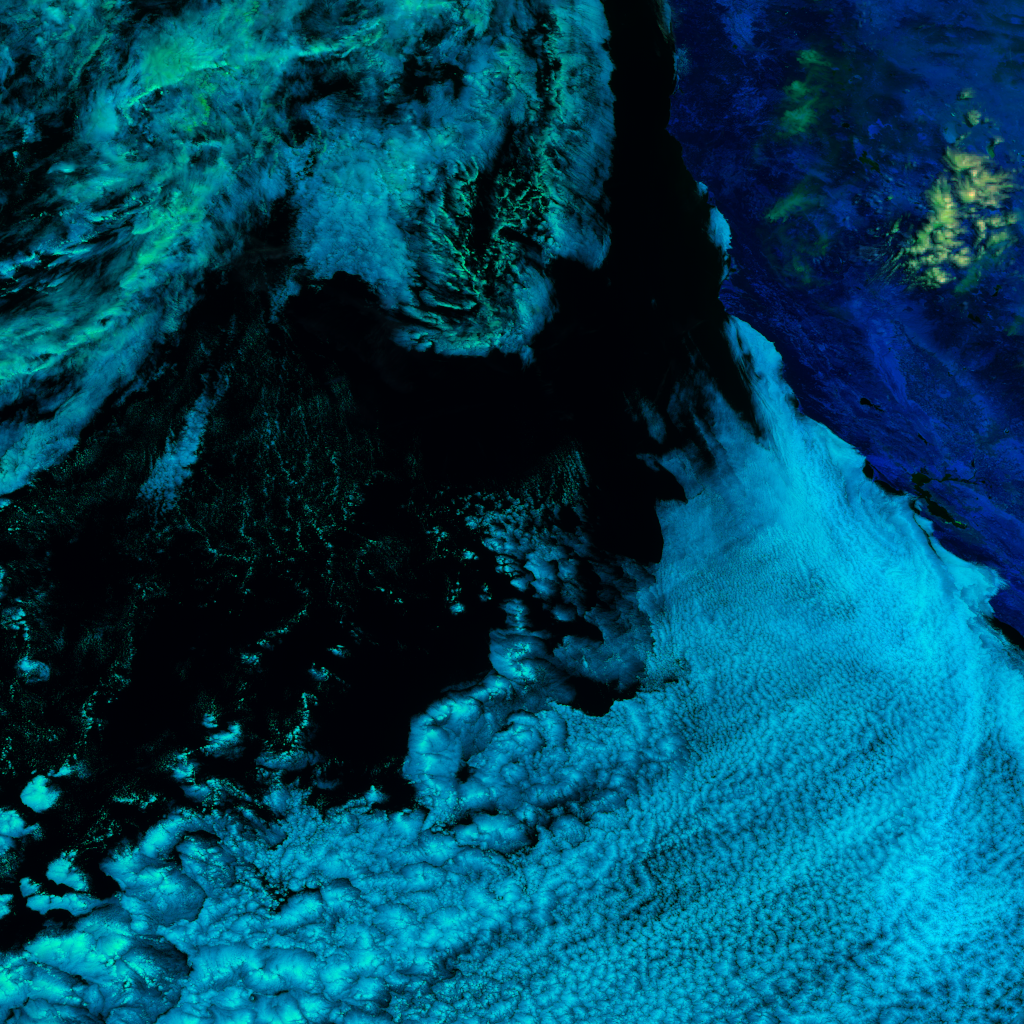
\includegraphics[width=.24\linewidth]{figs/abi_dcp_20210825-1918.png}
    \end{center}
    \caption{GOES ABI Day cloud Phase RGBs captured at a subset of the Terra and Aqua overpass times used in this report, showing the progression of the wildfires from August 18 (top left) to August 25 (bottom right). Light blue indicates warm water clouds, green indicates fine and uniform smoke particles, and red indicates cirrus cloud cover.}
\end{figure}


\section{Introduction}

    Clouds and aerosols both play a significant role Earth's radiation budget, but remain two of the greatest sources of uncertainty in modeling climate sensitivity \cite{masson-delmotte_climate_2021}. Clouds are difficult to characterize for several reasons including that they typically have conflicting longwave and shortwave effects that depend on the type and the temperature of both a cloud and the surface it occludes. Additionally, the feedback mechanisms that affect changes in the global distribution of clouds with respect to changing temperatures remain unclear \cite{ramanathan_cloud-radiative_1989}. Aerosols also pose challenges to modeling because (1) their type and distribution is highly regionally and contextually variable, (2) they can facilitate cloud nucleation (the so-called indirect effect), and (3) because they can enhance the evaporation rate of a juxtaposed cloud layer due to warming by absorption (semi-direct effect) \cite{kaufman_satellite_2002}. What's more is that in both cases there are no reliable counterfactual observations for comparing results to a pre-industrial atmosphere, which makes the anthropogenic contribution to climate forcing difficult to quantify. As such, it's especially important to employ direct observational data of clear skies, aerosols, and full-sky outgoing fluxes with broadband instruments like the Earth Radiation Budget Experiment (ERBE) constellation, and more recently CERES, which I employ in this report in order to estimate the radiative forcing due to clouds and aerosols over land and ocean surfaces.

    The setting for this study is a region covering the coast of central California over a 10-day period during a significant wildfire event. This is an appropriate choice for studying the radiative impact of clouds and smoke aerosols from biomass burning because the characteristic morning sea breeze consistently draws smoke aerosols out over the ocean, and facilitates the development of low-level stratocumulus clouds with a wide variety of optical depths. I restrict the data I use to only the daytime overpasses by Terra and Aqua, which are around 11:00am (19z) and 1:00pm (21z), respectively.

    For context, the 2021 California wildfire season was one of the worst on record, following a persistent drought that lasted throughout 2020 and until at least September of 2021. During this period of time, regional precipitation totals were the lowest since at least 1895 \cite{mankin_noaa_2021}, which culminated in 7,396 wildfires burning over 2,569,000 acres according to the California Wildfire Incident Archive \cite{the_department_of_forestry_and_fire_protection_2021_nodate}. Two of the most significant wildfire events were the Dixie and Caldor wildfires, which burned $963,309$ and $221,835$ acres respectively, mutually forced the evacuation of more than 29,000 residents, and were both the first known fires to cross the divide of the Sierra Nevada range \cite{chan_unprecedented_2021}\cite{the_department_of_forestry_and_fire_protection_2021_nodate}. The Caldor fire began conflagrating the High Sierra just West of Lake Tahoe on August 14 and rapidly grew over the following days, while the Dixie fire had already been burning further North since mid-July at the time of this study. These two forest fire events contributed much of the smoke considered in this study, and I personally witnessed the devastation and subsequent re-growth following the Caldor fire while backpacking the area in June 2023.


\section{Background: Satellites and Earth's Radiation Budget}

    \subsection{Early Satellite Retrievals of Outgoing Radiation}

    The first satellite observations of Earth's radiation budget were acquired by the low-resolution thermistor-based radiometers on board the TIROS-generation satellites between 1962 and 1966, and later by the similar ESSA III platform in 1966 and 1967 \cite{haar_measurements_1971}\cite{suomi_theoretical_1967}. The instruments simultaneously directly measured incoming solar irradiance, as well as rough outgoing broad-band radiance in the longwave and shortwave ranges \cite{house_radiation_1965}\cite{bartko_tiros_1964}. Early measurements from these platforms concluded in an estimated global mean albedo of $30\%$, and a global average longwave emission of $230.3\,\si{W.m^{-2}}$ \cite{house_radiation_1965}\cite{vonder_haar_satellite_1969}.

    \subsection{Earth's Radiation Budget Experiment}

    In the 1978, NASA launched the Nimbus 7 satellite carrying the first generation of the Earth's Radiation Budget (ERB) instrument, which enabled the development of a new methodology for retrieving accurate outgoing radiation estimates. This new strategy involves the co-location of narrow-FOV Advanced Very High Resolution Radiospectrometer (AVHRR) data with wide-FOV ERB data, and subsequently the use of angular distribution models (ADMs) to characterize surfaces and estimate the full-sky radiative flux of a surface from a radiance observation (with a particular Sun/surface/satellite geometry) \cite{taylor_reflectance_1984}\cite{jacobowitz_earth_1983}. The success of this mission was soon followed by the launch of 3 similar instruments, which flew aboard the NOAA-9, NOAA-10, and ERBS satellite platforms, which collectively form the Earth's Radiation Budget Experiment (ERBE) constellation \cite{barkstrom_earth_1984}.

    The advances in observational capacity as well as analysis techniques following the ERBE experiment facilitated the development of regional and seasonal estimates of Earth's radiation budget, which substantially enhanced understanding of the shortwave and longwave global energy balance \cite{breon_global_1994}. In particular, the juxtaposition of data from imagers having finer spatial and spectral resolutions enabled the scenes observed by broad-band instruments to be spectrally classified into surface types with common characteristics. This advancement led to the development of surface-specific bidirectional models (ADMs) for more accurate flux retrievals, as well as derivations of the radiative forcing by clouds as opposed to clear-sky \cite{ramanathan_cloud-radiative_1989}\cite{smith_inversion_1986}. The improved observations led to an updated average planetary albedo estimate of $31\%$, and an outgoing longwave radiation average of $235\,\si{W.m^{-2}}$ \cite{kiehl_earth_1997}.

    \subsection{Clouds and the Earth's Radiant Energy System}

    In 1997, NASA and the Japanese Aerospace Exploration Agency (JAXA) began collecting data with a new generation of broad-band instruments known as Clouds and the Earth's Radiant Energy System (CERES) launched on the Tropical Rainfall Measuring Mission (TRMM). This first instance of the instrument was limited in that TRMM didn't have global coverage, and CERES soon failed in August of 1998. Nonetheless, the NASA launched new versions of the instrument in 1999 and 2002 with the Terra and Aqua satellites as part of the Earth Observing System (EOS), which have proven extremely successful missions that presently continue to contribute valuable science data more than 20 years later.

    CERES is a 3-channel broadband radiometer that improves on ERB's measurement accuracy by up to a factor of 3, and offers a reduced sample FoV of about $16\times32\,\si{km}$. The three channels supported by CERES include $.2-5\mu m$ shortwave-range, $.2-100\mu m$ full-spectrum, and $8-12\mu m$ infrared window channels. Designers of the instrument neglected to include an independent longwave channel as a means of decreasing observation error due to material shortcomings, but accurate longwave estimates can be obtained by simply subtracting the shortwave instrument observations from those of the full-spectrum. The window channel is useful for estimating clear-sky surface fluxes as well as estimating the greenhouse effects of species with strong absorption outside the atmospheric window \cite{wielicki_clouds_1996}.

    In addition to the CERES instrument's improvements over ERB, the EOS satellite platforms include Moderate Resolution Imaging Spectroradiometer (MODIS) imagers with a wealth of narrow-band channels co-located with the CERES observations. These substantially enhance the quality of spectral classification and material retrievals from within a CERES FoV (hereafter referred to as a footprint). These help supplement CERES data with high-quality information about surface types and the properties/distribution of atmospheric materials. Additionally, Terra and Aqua include a second CERES instrument (in addition to the typical one scanning in a cross-track mode) which spins azimuthally in order to contribute near-simultaneous observations of surfaces from a second viewing angle. Data from the second instrument is critical for producing accurate and empirical ADMs.

    \section{Converting CERES Radiance to TOA Flux}

    \subsection{Filtered to Unfiltered Radiance}

    The first step to determining the TOA flux from broadband observations of radiance by the CERES instrument is to remove the effect of the instrument's relative spectral response function (RSR). As with any physically realistic radiometer, the digital counts recorded by the instrument are somewhat spectrally dependent on the wavelength of incident light. Since radiation budget experiments seek to observe the actual magnitude of energy associated with outgoing radiation, as opposed to relative magnitudes that are often sufficient for imager applications, it is critically important to correct for the error caused by the instrument's imperfect spectral sensitivity.

    In general, the observed radiances can be thought of as a filter convolution of the RSR function over the actual surface's radiance, which is a fundamentally information-lossy process. Thus, ``undoing'' this effect is neccesarily an approximation. In the case of CERES, this involves estimating so-called \textit{unfiltered} radiance in each channel in terms of emperically-derived coefficients, which form linear combinations of the filtered radiances. These coefficients depend on each footprint's surface class as well as the viewing geometry, and are sometimes be periodically updated throughout the instrument's lifetime \cite{loeb_determination_2001}.

    \subsection{Angular Distribution Models}

    As mentioned in the previous section, one of the major advancements that enables accurate characterization of top-of-atmosphere fluxes are angular distribution models, or ADMs, which seek to represent the dependence of the observed radiance of a particular scene type on the viewing geometry. Broad-band imagers on satellite platforms can only ever observe \textit{radiances} in $\si{W.m^{-2}.sr^{-1}}$ since they necessarily have a specific position with respect to the surface they are observing. This poses a challenge for the retrieval of the full-sky radiant flux of a surface, because the absorbed or emitted radiation may be strongly anisotropic. This challenge is even more prominent for instruments with a relatively large footprint such as CERES because the incident surface type may be highly variable. As such, there is a need for careful modeling of the dependence of observed radiance on viewing angle.

    \begin{equation}\label{toa-flux}
        F(\theta_0) = \int_0^{2\pi} \int_0^{\frac{\pi}{2}} I(\theta_0, \theta, \phi) \, \cos(\theta) \, \sin(\theta) \, d \theta \, d \phi
    \end{equation}

    Equation \ref{toa-flux} expresses the full-sky TOA flux $F(\theta_0)$ given solar zenith angle $\theta_0$ with respect to radiance $I$, viewing zenith angle $\theta$, and viewing azimuth angle $\phi$. Once a surface type has been identified for a footprint (typically using spectral/spatial classification of co-located imager data), the task of that surface's ADM is to provide a discrete estimate of the above integral in terms the footprint's $(\theta_0, \theta, \phi)$ configuration. This estimate takes the form of a lookup table value known as an \textit{anisotropic factor} $R_s$.

    \begin{equation}\label{aifac}
        R_s(\theta_0, \theta, \phi) \approx \pi\frac{\overline{I}_s(\theta_0, \theta, \phi)}{\overline{F}_s(\theta_0) } \,\,\, \Rightarrow \,\,\,
         F_s(\theta_0) \approx \pi\frac{I_s(\theta_0, \theta, \phi)}{R_s(\theta_0, \theta, \phi)}
    \end{equation}

    Equation \ref{aifac} shows how the anisotropic factor $R_s$ for surface $s$ is estimated, and subsequently how it can be used to approximate the full-sky flux. On the left hand side, the anisotropic factor is approximated as the ratio of the mean isotropic radiance $\pi\,\overline{I}_s(\theta_0, \theta, \phi)$ within an angular bin to the surface's average full-sky-flux $\overline{F}_s(\theta_0)$. Since the fundamental problem here is that $\overline{F}_s(\theta_0)$ can't be directly observed, its value is estimated using large ensembles of observations, which will ideally converge on reliable values per angular bin, if surface classes are selected well. Once lookup tables of anisotropic factors have been empirically determined for a surface, they are applied to scale actual radiance observations $I_s(\theta_0, \theta, \phi)$ into estimates of TOA flux $F_s(\theta_0)$ \cite{suttles_angular_1988}\cite{su_next-generation_2015}\cite{loeb_angular_2005}.

    An additional consideration that must be taken into account while constructing angular dependence models is the TOA reference level used when modeling outgoing fluxes. This is not normally a consideration that must be made for imager data, which is supposed to correspond to radiance emerging directly from the observed surface, however for large-footprint flux calculations it becomes important to consider the influence of radiance corresponding to secant ``slant paths'' through the atmosphere but above the observed surface. Changing the reference height essentially just modifies the surface area over which outgoing radiation is presumed to be distributed, however for CERES-sized footprints, this can be responsible for an error of a few $\si{W.m^{-2}}$ of flux associated with the observed surface. The ideal TOA reference height determined for the CERES ADMs is $z_{TOA} = 20\,\si{km}$, as identified by (Loeb, 2002)\cite{loeb_defining_2002}.

    \begin{multicols}{3}
        \begin{enumerate}[itemsep=0pt, parsep=0pt, before=\setlength{\baselineskip}{6mm}]
            \item \textbf{Evergreen Needleleaf}
            \item Evergreen Broadleaf
            \item Deciduous Needleleaf
            \item \textbf{Deciduous Broadleaf}
            \item Mixed Forest
            \item Closed Shrubland
            \item \textbf{Open Shrubland}
            \item \textbf{Woody Savannas}
            \item \textbf{Savannas}
            \item \textbf{Grassland}
            \item Permanent Wetland
            \item \textbf{Cropland}
            \item \textbf{Urban/Industrialized}
            \item \textbf{Cropland Mosaic}
            \item Permanent Snow/Ice
            \item Exposed Soil/Rock
            \item \textbf{Water Bodies}
            \item Tundra
            \item Fresh Snow
            \item Sea Ice
        \end{enumerate}
    \end{multicols}

    The ADMs used for retrieving fluxes from CERES data are separated into the 20 surface types shown above, of which only the bolded items are considered in this report. Although there are some footprints in the RoI identified as urban/industrialized or fresh snow in the data I acquired, they did not meet the thresholded requirements for consideration in my energy budget calculations.

    \subsection{Co-location of Imager Data}

    \begin{equation}\label{psf-prop}
        \overline{x} = \frac{\int_{FOV} P(\delta,\beta)\,x(\delta,\beta)\,\cos(\delta)\,d\beta\,d\delta}{\int_{FOV} P(\delta,\beta)\,\cos(\delta)\,d\beta\,d\delta}
    \end{equation}

    As mentioned in previous sections, an accurate assessment of the TOA flux at CERES' footprint resolution requires careful co-location of spatially and spectrally finer-resolution pixel data from the on-board MODIS radiometer. CERES' sensitivity to radiance within a footprint is not constant throughout the footprint area due to the nonzero exposure time of a pixel, the translational motion of the satellite, as well as inherent instrument properties. Thus, in order to appropriately estimate the influence of the properties retrieved from imager data on the flux observations by CERES, the sensor's point spread function (PSF) $P(\delta,\beta)$ must be considered with respect to orthogonal viewing angles $\delta$ and $\beta$ within a single footprint. Equation \ref{psf-prop} is the continuous form of the expression used estimate the PSF-weighted average value of an imager pixel property $\overline{x}$ within a footprint's $FOV$. This spatial averaging technique is used in the generation of CERES SSF data in order to produce full-footprint averages of cloud/aerosol optical depth, percent coverages of incident surface types, estimates of cloud top temperature/pressure, and other useful metrics derived from MODIS radiances.

    \section{Forcing Theoretical Basis}

    \begin{equation}\label{rad-heat}
        H = S(1-\alpha) - F^{(\uparrow)}_{LW} = F^{(abs)}_{SW} - F^{(\uparrow)}_{LW}
    \end{equation}

    The climate forcing attributable to an atmospheric component such as clouds or aerosols is a function of the material's influence on incoming shortwave solar radiation, as well as its effect on emitted longwave radiation. As such, in the most general form, the net radiative heating of an atmospheric column can be expressed in terms of the difference between the absorbed shortwave radiation within the column, and its outgoing longwave emissions, as demonstrated by Equation \ref{rad-heat}.

    Since clouds and aerosols are transient phenomena with radiation effects that depend on other properties such as optical depth, single scatter albedo, and effective radius, it's helpful to express their forcing effect in terms of the variation in the net heating of an atmospheric column containing the cloud or aerosol from that of the same atmospheric column without the cloud or aerosol. Given a clear-sky heating rate $H$ as shown above, and the heating rate given the presence of a cloud $H_{cld}$, the total climate forcing as a consequence of the cloud (i.e. cloud radiative forcing) is determined to be $CRF = H_{cld} - H$. Similarly, given the heating rate of an aerosol-laden atmospheric column $H_{aer}$, the aerosol radiative forcing is $ARF = H_{aer} - H$.

    The above expressions for CRF and ARF are structured such that positive values are associated with a net heating effect from clouds or aerosols, and negative values indicate net cooling within the atmosphere. It's also critical to note that the clear-sky heating $H$ in both cases is highly dependent on the incident surface, and even the relative heating rates in the presence of clouds or aerosols can depend on the surface type in a nonlinear fashion due to feedback mechanisms. Therefore in this project I calculate the atmospheric forcing effects of clouds and aerosols independently for each surface type represented in the RoI.

    \section{Cloud and Aerosol Forcing Results}

    \subsection{Methodology}

    The CERES SSF dataset I used for this assignment contains a wealth of information associated with each footprint, which makes it straightforward to set thresholds based on sub-footprint imager data and satellite geometric configuration, and to independently consider surfaces based on their type class and consistency. Aerosol-cloud interactions and the radiative forcing over highly heterogeneous surfaces are out of the scope of this project, so I generally restricted the footprints I used to exclude those with aerosols and clouds in close proximity, those with any high-level cirrus contamination, and those containing inconsistent surface types. As an exception, due to the scarcity of some valid samples and similarity in their observed radiative forcing curves, I merged (1) Evergreen Needleleaf and Deciduous Broadleaf classes into a single class for all Forests, (2) Savannas, Woody Savannas, and Grassland classes into a single class for Savanna, and (3) Cropland and Cropland Mosaic classes into a single class for Crops.

    The following constraints were imposed on the footprints used in each flux forcing calculation, as defined in (Loeb, 2018) \cite{loeb_503_2018}.

    \noindent
    \textbf{Cloud Optical Depth Constraints}
    \begin{itemize}[itemsep=0pt, parsep=0pt, before=\setlength{\baselineskip}{6mm}]
        \item Standard deviation of COD of imager pixels less than $10$
        \item Upper bound of $2\%$ of imager pixels identified as containing aerosols
        \item At least $80\%$ of imager pixels identified as the dominant surface class
    \end{itemize}

    \textbf{Aerosol Optical Depth Constraints}
    \begin{itemize}[itemsep=0pt, parsep=0pt, before=\setlength{\baselineskip}{6mm}]
        \item At least $80\%$ of imager pixels identified as the dominant surface class
    \end{itemize}

    \begin{figure}[h!]\label{flux-interp}
        \centering
        \begin{center}
            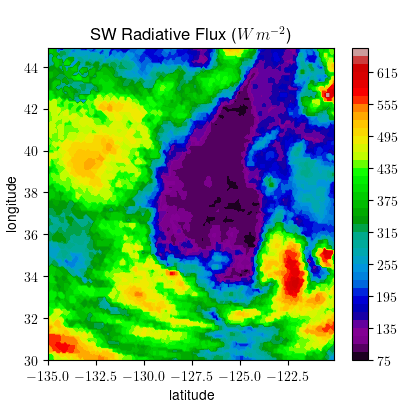
\includegraphics[width=.48\linewidth]{figs/interp_swflux.png}
            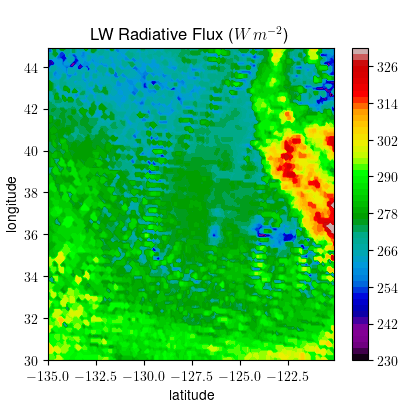
\includegraphics[width=.48\linewidth]{figs/interp_lwflux.png}
        \end{center}
        \caption{Outgoing Shortwave and Longwave fluxes observed by CERES on August 18, 2021 at 1910z (same swath as Figure \ref{cover}). The $\sim16\times32\,\si{km}$ footprints are resampled onto a uniform $0.1^\circ$ grid by nearest-neighbor interpolation.}
    \end{figure}

    \subsection{Cloud Radiative Forcing}

     Clouds have a substantial influence on the radiation budget due to their high reflectivity as well as emissivity. In the shortwave range, enhanced reflection of insolation causes a general cooling effect that is most prominent in the mid-latitude summer, and over bodies of water \cite{harrison_seasonal_1990}. This effect is clearly demonstrated by the broad-band shortwave flux in Figure \ref{flux-interp}, which shows that outgoing shortwave radiation over the highest-reflectivity water clouds exceeds that of the ocean surface by as much as $540\,\si{W.m^{-2}}$.

    The longwave impact of clouds is less prominent for liquid water clouds over the ocean since both surfaces have a comparable temperature and emissivity, however over land (in the top right of the second image in Figure \ref{flux-interp}), there is a stark depression in outgoing longwave radiation (OLR) associated with low-level water clouds. Furthermore, the thin cirrus clouds associated with red hues in the center-right of Figure \ref{cover} correspond to a decrease in OLR over the same area in Figure \ref{flux-interp}. Both of cases are indicative of the greenhouse effect of clouds which result in a net warming effect that is generally less prominent than the shortwave forcing.

    \subsection{Aerosol Radiative Forcing}

\begin{table}[h!]
    \centering
    \begin{tabular}{ m{.15\linewidth} | m{.15\linewidth} | m{0.6\linewidth}}
        \textbf{Parameter} & \textbf{Value} & \textbf{Justification} \\
        \hline
        & & \\
    \end{tabular}
    \caption{}
    \label{}
\end{table}

\section{Retrieval Methodology}

\subsection{Model Analysis}

\begin{figure}[h!]
    \centering
    \begin{center}
        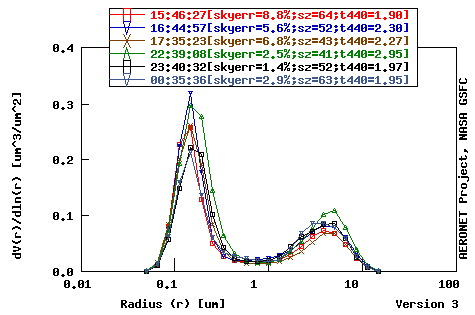
\includegraphics[width=.55\paperwidth]{figs/20210818_aeronet_ames_sdist.png}
        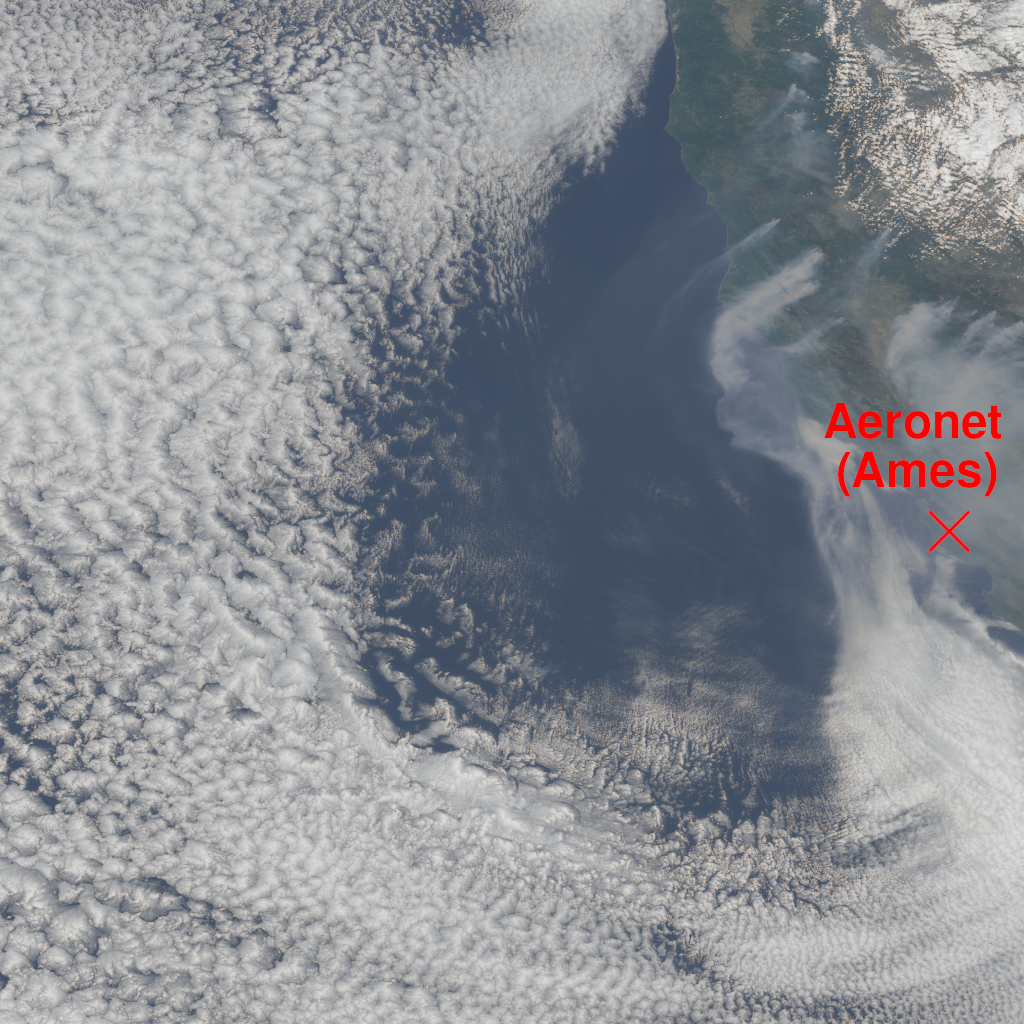
\includegraphics[width=.55\paperwidth]{figs/20210818_aeronet_marked-rgb.png}
    \end{center}
    \caption{}
    \label{}
\end{figure}

\subsection{Reference Pixel Selection}


\subsection{Aerosol Optical Depth Retrieval}

\section{Results}

\subsection{Validation Comment}

\subsection{Analysis}

\begin{table}[h!]\label{}
    \centering
    \begin{tabular}{ c c | c c c c c}
        & & & & & & \\
        \hline
        \multirow{4}*{} &
        & & & & & \T\\
        & & & & & \B\\
        \hline
        \multirow{2}*{Valid} &
        Meta & .2779 & .246 & .3684 & .4755 & .3923 \T\\
        &Grid & .2791 & .2495 & 2.270 & 2.378 & 2.292 \B\\
    \end{tabular}
    \caption{Comparison between my retrieval results and AOD values reported in the DESIS metadata, as well as the pixels in the AOD tiff grid corresponding to DDV values.}
\end{table}

%\end{multicols}

\section{Conclusion}

\bibliography{main}

\end{document}
